\chapter{算法渐进分析}

\begin{introduction}
   \item 渐进记号
   \item 渐进增长的性质
   \item 常见的渐进函数
\end{introduction}

\section{关于算法的计算效率}
当我们在了解计算效率或者研究算法的复杂度时,我们主要集中于运行算法的时间效率
--因为我们总是希望能够更快地运行算法。当然对于空间复杂度也是不能够忽略的,
不过一下我们主要以算法的时间复杂度为载体,介绍算法的渐进分析,空间复杂度的分析
可以进行类比。
 
一个算法在规模为n的输入下,最坏情况运行时间增长率最多与某个函数$f(n)$成正比,
函数$f(n)$因此就成为了我们算法运行时间的一个界限,下面将对此进行详细讨论。
 
\section{\texorpdfstring{$O,\ \Omega,\ and\ \Theta $}{O, Ω, and θ}}
在这里,我们希望寻找一种表达算法时间复杂或者是其他函数的方法,在这种方法中,常数系数和低次项
对结果是没有影响的。比如 $1.62n^2+3.5n+2.3$ 增长的方式和 $n^2$ 一样。

\begin{figure}[h]
   \begin{minipage}[t]{1\linewidth}
      \centering
      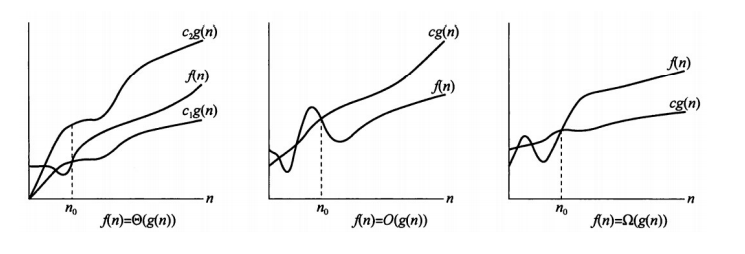
\includegraphics[width=10cm,height=3.5cm]{image/asymptotic_analysis_1.png}
      \caption{$O,\ \Omega,\ and\ \Theta $}
   \end{minipage}
\end{figure}
 
\subsection{渐进上界 $O$}
令$f(n)$为算法在输入规模为n的情况下的运行时间(最坏情况),给定另一个函数$g(n)$,当n充分大,
函数$f(n)$不会超过$g(n)$的常数倍,就有$f(n)=O(g(n))$。数学定义如下:

\begin{definition}{O ($\cdot$)}{def1}   
   \[    
   O(g(n))= \{f(n): \exists\ c,n_0\in R^+,such\ that: \forall n\ge n_0:0\le f(n)\le cg(n)\} 
   \]
\end{definition}
   

举个例子作为说明,假设算法的运行时间有着$f(n)=pn^2+qn+r$的形式,其中p,q,r均为正常数,我们可以说
任何具有这种形式的函数都是$O(n^2)$即$pn^2+qn+r=O(n^2)$ ,证明如下:
\begin{proof}
   \begin{align*}
      \forall n \geq 1,t&hen\ qn\leq qn^2,r\leq rn^2 \\
      \Longrightarrow   f(n)&=pn^2+qn+r \\
      &\leq pn^2+pn^2+rn^2\\
      &=(p+q+r)n^2
   \end{align*}
\end{proof}
注意到$O(\cdot)$仅仅代表一个上界,并不代表函数准确的增长率,例如$pn^2+qn+r=O(n^3)$也是成立的
但是它不是“最紧”的一个上界。
\subsection{渐进下界\ $\Omega$}
对于算法的渐进下界,我们同样可以对其进行说明:令$f(n)$为算法在输入规模为n的情况下的运行时间,给
定另一个函数$g(n)$,如果对充分大的n,函数$f(n)$至少是函数$g(n)$的常数倍,就有$f(n)=\Omega(g(n))$
\begin{definition}{$\Omega(\cdot)$}{def2}
\[
   \Omega (g(n))= \{f(n): \exists\ c,n_0\in R^+,such\ that: \forall n\ge n_0:0\le cg(n)\le f(n)\}
\]
\end{definition}

继续使用 $f(n)=pn^2+qn+r$ 的例子,其中q 、p、 r 均为正常数,我们可以说具有任何这种形式的函数都是$\Omega(n)$。
证明如下:
\begin{proof}
   \begin{align*}
      \forall n \geq 1,t&hen\ qn\leq 0,r\geq 0 \\
      \Longrightarrow   f(n)&=pn^2+qn+r \\
      &\geq pn^2+pn^2+rn^2\\
      &=(p+q+r)n^2
   \end{align*}
\end{proof}

同$O(\cdot)$的情况,我们注意到$\Omega(\cdot)$仅仅代表一个下界,例如:$f(n)=pn^2+qn+r=\Omega(n)$也是成立的。

\subsection{渐进紧界$\Theta$}
在上面知识的支持下,我们发现,对于同一个$f(n)$,其上下界,所对应的$g(n)$可能是相同的,即$f(n)=O(g(n))$并且$f(n)=\Omega(g(n))$
,在这种情况下,我们可以说$f(n)=\Theta(g(n))$
\begin{definition}{$\Theta(\cdot)$}{def3}
   \[
      \Theta(g(n)) = \{f(n): \exists\ c_1,c_2,n_0\in R^+,such\ that: \forall n\ge n_0:0\le c_1 g(n)\le f(n)\le c_2 g(n)\}
   \]
\end{definition}

沿用刚才的例子,对于$f(n)=pn^2+qn+r$,我们可以说任何具有该
形式的函数都是$\Theta(n^2)$的,对于其证明就再简单不过了,我们只需要将上面两段合起来即可!
在实际的计算中,对于显示的函数,我们为了求得$\Theta(\cdot)$,只需保留其最大幂的多项式或者主要成分,去掉常数项即可。
\\
\\
除了刚刚介绍的方法,我们还可以利用以下性质求得$\Theta(\cdot)$:
\\
设$f$和$g$是两个函数,并且
\[
   \lim_{n\rightarrow+\infty}\frac{f(n)}{g(n)} = c \ (c\ge 0)
\]
那么$f(n)=\Theta(g(n))$,关于该部分的证明,留给读者自行探索。


\section{渐进增长的一些性质}
下面将给出渐进增长的一些性质,对于性质的证明,可以自己证明一下,然后与《Algorithm\ Design》的P38\~P40的证明进行对照
\begin{theorem}{Transitivity}{}
   (a)\ If\ $f=O(h)$\ and\ $g=O(h)$, then $f=O(h)$\\
   (b)\ If\ $f=\Omega(h)$\ and\ $g=\Omega(h)$, then $f=\Omega(h)$\\
   (c)\ If\ $f=\Theta(h)$\ and\ $g=\Theta(h)$, then $f=\Theta(h)$
\end{theorem}

\begin{theorem}{Sum\ of\ Functions}{}
   假设$f$和$g$是两个函数,若对某个其他的函数$h$,都有:$f=O(h),g=O(h)$\\
   那么,$f+g=O(h)$\\
   推广开来:令k是确定的常数,$f_1,f_2,f_3,\cdots,f_k$和$h$是函数,且
   $f_i=O(h)$ \ \ $i\in (1,k)$,\\
   那么,$\sum^{k}_{i=1}f_i=O(h)$
\end{theorem}

\begin{theorem}{ }{}
   假设$f$和$g$是两个函数,(取非负值),使得$g = O(f)$\\
   那么$f+g=\Theta(f)$
\end{theorem}

\section{常见的渐进函数}
在一般的算法复杂度的分析中,我们常使用$O(\cdot)$进行渐进分析,其中常用的函数有以下几个:\\
算数级复杂度:
$$
O(1)<O(logn)<O(n)<O(nlogn)<O(n^2)<O(n^2logn)<O(n^3)< \cdots
$$

指数级复杂度:
$$
O(2^n)<O(n!)<O(n^n)
$$
如要了解更多的标准记号和常用函数,可以参考算法导论P30-P34